\documentclass{scrartcl}

%%%%%%%%%%%%%%%%%%%%%%%%%%%%%%%%%%%%%%%%%%%%%%%%%%%%%%%%%%%%%%%%%%%%%%%%%%
% CUSTOM VARIABLES (CHANGE THESE TO YOUR NEED)
%%%%%%%%%%%%%%%%%%%%%%%%%%%%%%%%%%%%%%%%%%%%%%%%%%%%%%%%%%%%%%%%%%%%%%%%%%
\newcommand{\myname}{Leonard Rienks}
\newcommand{\mymatriclenum}{5154774}
\newcommand{\partnername}{Leonard Rienks}
\newcommand{\partnermatriclenum}{5154774}
\newcommand{\lecture}{Some random lecture}
\newcommand{\exercise}{Exercise X}
%\newcommand{\groupnum}{My group} - potential additions
%\newcommand{\tutor}{My tutor}

\newcommand{\mytitle}{\exercise}
\newcommand{\mysubtitle}{\lecture}
\newcommand{\myauthor}{\myname, \partnername}

%%%%%%%%%%%%%%%%%%%%%%%%%%%%%%%%%%%%%%%%%%%%%%%%%%%%%%%%%%%%%%%%%%%%%%%%%%
% EVERY TIME PACKAGES (JUST USE THEM) AND DEFINITIONS (CHANGE THESE TO YOUR NEED) 
%%%%%%%%%%%%%%%%%%%%%%%%%%%%%%%%%%%%%%%%%%%%%%%%%%%%%%%%%%%%%%%%%%%%%%%%%%

%%%%%%%%%% Layout Support %%%%%%%%%%
\usepackage{fancyhdr}
\usepackage{geometry}
\usepackage[shortlabels]{enumitem}  % For customizing and controlling the appearance and behavior of lists, such as itemized lists, enumerated lists, and description lists
\geometry{a4paper, left=2.5cm, right=2.5cm, top=3.5cm, bottom=2.5cm}  % Adjust margins, paper size etc. with a more special package
\fancypagestyle{mystyle}{  % all non-defined settings default to the "fancy" style from the fancyhdr package
    \setlength{\headheight}{30pt}
    \setlength{\headwidth}{\textwidth}
    \setlength{\headsep}{13pt}          % The separation between the header and the main text body
    \renewcommand{\headrulewidth}{0.4pt}
    \renewcommand{\footrulewidth}{0.4pt}
    \setlength{\footskip}{23pt}
    \setlength{\topmargin}{0pt}
    \setlength{\oddsidemargin}{0pt}     % Change to have a difference between odd and even page margins (when the document is printed in a book format)
    \setlength{\evensidemargin}{0pt}
    \setlength{\marginparwidth}{50pt}   % The width of the margin notes area
    \setlength{\marginparsep}{7pt}      % The separation between margin notes and the main text
    \setlength{\textwidth}{468pt}       % width of the main text area
    \setlength{\textheight}{648pt}
}
% \KOMAoptions{paper=a4, fontsize=12pt}  % Set the paper size and font size.
% \setkomafont{section}{\Large\rmfamily}  % Adjust the font size and style for section titles
% \renewcommand*{\sectionformat}{\thesection\autodot\enskip}  % Customizes the format of section numbers.
\usepackage{placeins} 			% For better Handling of floats
\usepackage{float}
\usepackage{subcaption}
\captionsetup{format=plain}
\captionsetup{labelfont=bf}
%\usepackage[tight,footnotesize]{subfigure} % EITHER THIS OR SUBCAPTION
\usepackage[  % Hyperlinks and PDF Metadata
pdftex,
pdfauthor={\myauthor},
pdftitle={\mytitle},
pdfsubject={Uni Freiburg},
pdfkeywords={}]
{hyperref}
\hypersetup{colorlinks=true, citecolor=black, linkcolor=black, urlcolor=blue}

%%%%%%%%%% Title %%%%%%%%%%
\author{\myauthor}
\title{\mytitle}
\subtitle{\mysubtitle}

%%%%%%%%%% Heading and Footing %%%%%%%%%%
\pagestyle{mystyle}
\fancyhf{}  % Clear the header and footer settings
\lhead{  % Define a header from the left, same as \fancyhead[L]{}
\begin{tabular}{ll}     % CHANGE THIS HEADER TO YOU YOUR LIKING
\myname & \mymatriclenum \\
\partnername & \partnermatriclenum \\
\end{tabular}
}
% \fancyhead[EL]{} % E for even, O for odd to define different headers and footers for even and odd pages
\rhead{\today}  % Define a header from the right
\chead{\mytitle}
\cfoot{Page \thepage}  % Define a footing in the center

%%%%%%%%%% Language support %%%%%%%%%%
\usepackage[main=english, ngerman]{babel} % switch for German version
\usepackage[utf8]{inputenc}
\usepackage[T1]{fontenc} % Improved support for german-specific letters (Umlaute)

%%%%%%%%%% Math support %%%%%%%%%%
\usepackage{amssymb}  % For additional symbols
\usepackage{amsmath}  % For enhanced mathematics typesetting

%%%%%%%%%% Include Support %%%%%%%%%%
\usepackage{graphicx}
\usepackage{pdfpages}


%%%%%%%%%%%%%%%%%%%%%%%%%%%%%%%%%%%%%%%%%%%%%%%%%%%%%%%%%%%%%%%%%%%%%%%%%%
% SITUATIONAL PACKAGES AND DEFINITIONS (COPY WHAT YOU NEED)
%%%%%%%%%%%%%%%%%%%%%%%%%%%%%%%%%%%%%%%%%%%%%%%%%%%%%%%%%%%%%%%%%%%%%%%%%%

%%%%%%%%%% General %%%%%%%%%%
\usepackage{xcolor}             % For extra color definitions
\definecolor{codegreen}{rgb}{0,0.6,0}  % A few examples, feel free to experiment
\definecolor{codegray}{rgb}{0.5,0.5,0.5}
\definecolor{codepurple}{rgb}{0.58,0,0.82}
\definecolor{backcolour}{rgb}{0.95,0.95,0.92}
\usepackage{tikz}				% For drawing anything
\usepackage{tikzsymbols}
\usepackage{chngcntr}           % To control the numbering and formatting of counters in your document
\usepackage{dirtytalk}          % easier use of quotation marks with \say{This is a quoted text.}
\usepackage{datetime}
\usepackage{advdate}            % to automatically specify dates in the future

%%%%%%%%%% Tables %%%%%%%%%%
\usepackage{booktabs}			% For nicer tables
\usepackage{multirow}			% Connect rows and columns in your tables
\usepackage{array}              % Idk

%%%%%%%%%% Scientific writing %%%%%%%%%%
\usepackage{siunitx}            % For consistent and easy Unit usage
\sisetup{
  locale = DE
%, exponent-product = \cdot      % Definition of , and . usage
}
%\DeclareSIUnit\torr{Torr}       % Declaration of additional units
%\DeclareSIUnit\sccm{sccm}       % Declaration of additional units
\usepackage{pgfplots}           % For making plots
\pgfplotsset{width=7cm,compat=1.9}       % Version
\usepackage{pgf-pie}            % For pie-charts
\usepackage{mathtools}          % MORE math symbols and tools
\usepackage{mathabx}

%%%%%%%%%% Referencing %%%%%%%%%%
\usepackage{csquotes}
\usepackage[sorting=none]{biblatex} % Best in combination with Zotero
\addbibresource{Sources/topic.bib}

%%%%%%%%%% Code-Listings %%%%%%%%%%
\usepackage{listings}
\lstset{
    basicstyle=\ttfamily\scriptsize,
    keywordstyle=\color{blue},
    commentstyle=\color{green!40!black},
    stringstyle=\color{red},
    numbers=left,
    numberstyle=\small,
    numbersep=7pt,
    breaklines=true,
    frame=single,
    captionpos=b,
}

%%%%%%%%%% Tikz symbol commands %%%%%%%%%%
% Controller Button symbols
\newcommand{\controllerbutton}[1]{
  \raisebox{-0.22cm}{
    \begin{tikzpicture}
      \draw (0,0) circle [radius=0.3cm];  % Outer circle
      \filldraw (0,0) circle [radius=0.25cm];  % Inner circle (button)
      \node at (0,0) [text=white] {#1};  % Label with the provided letter in white color
    \end{tikzpicture}
  }
}



%%%%%%%%%%%%%%%%%%%%%%%%%%%%%%%%%%%%%%%%%%%%%%%%%%%%%%%%%%%%%%%%%%%%%%%%%%
% ACTUAL DOCUMENT (COPY WHAT YOU NEED)
%%%%%%%%%%%%%%%%%%%%%%%%%%%%%%%%%%%%%%%%%%%%%%%%%%%%%%%%%%%%%%%%%%%%%%%%%%

% Pre-Amble (usually worth to just copy)
\begin{document}
\counterwithin{figure}{section}
\counterwithin{table}{section}
\counterwithin{equation}{section}
\counterwithin{lstlisting}{section} % only needed when using lstlistings

\maketitle
\thispagestyle{empty} % Exclude page number from title page
\tableofcontents  % optional if your document is small
\thispagestyle{empty} % Exclude page number and header from table of contents
\newpage
\setcounter{page}{1}

\section{Organization}
\subsection{Listings}
\subsubsection{Itemize}
\begin{itemize}
    \item Creates simple bullet points, quick and straightforward
\end{itemize}
\subsubsection{Enumerate with parameters (with the enumitem package)}
\begin{enumerate}[label=\alph*)]
    \item Allows simple configuration of enumeration symbols according to your needs
    \item Probably the best choice in most cases
\end{enumerate}

\section{Additional Formatting}
\subsection{Fonts}
\subsubsection{Standard Variants}
\begin{itemize}
    \item \textbf{TextBF:} Simply select text, press Ctrl+B, and the text will be bolded
    \item $\text{Math mode: } \int_{0}^{\pi} \sin(x) \, dx = 2$ for all mathematical symbols ($\sum$) / expressions ($s_2$). Can be either closed or interrupted with the text command for text.
    \item \texttt{TextTT:} For instance, useful for lecture-specific definitions
\end{itemize}
\subsection{Colors}
For this, it is best to use the Xcolor package. In addition to standard colors or custom-defined colors (see Situational Definitions), specific RGB or HTML colors can be called ([red] $\to$ [RGB]{255,0,0}). Usable for both regular text and Math mode: \textcolor[RGB]{255,0,0}{Example $s_{42}$}
\begin{itemize}
    \item \textcolor[RGB]{100,100,100}{Textcolor}
    \item \colorbox{codegreen}{Colorbox}
\end{itemize}

\section{Equations}
\subsection{Simple Equation with equation}
Here is the simple equation \ref{eq:amp}
\begin{equation}
\label{eq:amp}
 R_{17}=\frac{V_{MP58}\cdot (R_{17}+R_{65})}{V_{MP53}} = \frac{\SI{0.66}{\volt}\cdot (R_{17}+\SI{10}{\kilo\ohm})}{\SI{5}{\volt}}=\SI{1520.74}{\ohm}
\end{equation}
Here is one with matrices (see equation \ref{eq:Matrices}):
\begin{equation}
\label{eq:Matrices}
A_3*A_4=
    \left(\begin{array}{ccc}
         0&-1&-2\\
         -1 & 0&1\\
         2 & 1& 0
    \end{array}\right)
    *
    \left(\begin{array}{cc}
         1 & -1\\
         -2 &2\\
         3 & -1
    \end{array}\right)
    =
    \left(\begin{array}{cc}
         -4 & 0\\
         2 & 2\\
         0 & -4
    \end{array}\right)
\end{equation}
\subsection{Multiline Equations with align}
Here is the multiline equation \ref{eq:VoltageDivider_PT1000} with align
\begin{align}
\label{eq:VoltageDivider_PT1000}
    R_{17}&=\frac{(R_{73}+POT_1)\cdot(R_{17}+R_{65})}{R_{73}+POT_1+R_{64}}\\
    \equiv R_{17}&=\frac{(R_{73}+POT_1)\cdot R_{65}}{R_{64}}\\
    &=\frac{\SI{0.866}{\kilo\ohm}\cdot\SI{10}{\kilo\ohm}}{\SI{8.2}{\kilo\ohm}}=\SI{1056.1}{\ohm}
\end{align}
\subsection{Complete Induction}

\section{Figures}
\subsection{Simple Graphic}
Here is the graphic \ref{fig:AutumnCatch}
\noindent
\FloatBarrier
\begin{figure}[ht]
    \centering
    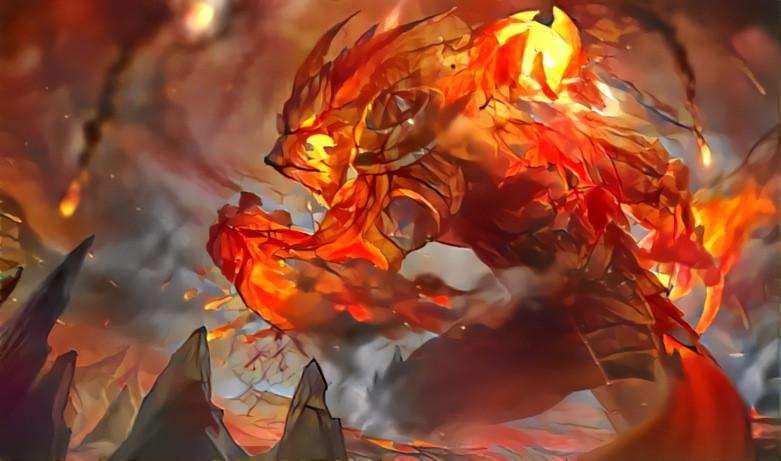
\includegraphics[width=0.4\textwidth]{Graphics/Herbstfang.jpg}
    \caption{Some picture}
    \label{fig:AutumnCatch}
\end{figure}
\FloatBarrier
\noindent
\subsection{Multiple Graphics}
And here are the graphics \ref{fig:AutumnCatch2}, \ref{fig:AutumnCatch3}, and \ref{fig:AutumnCatch4} using a minipage.
\FloatBarrier
    \noindent
\begin{figure}[H]
        \minipage{0.32\textwidth}
  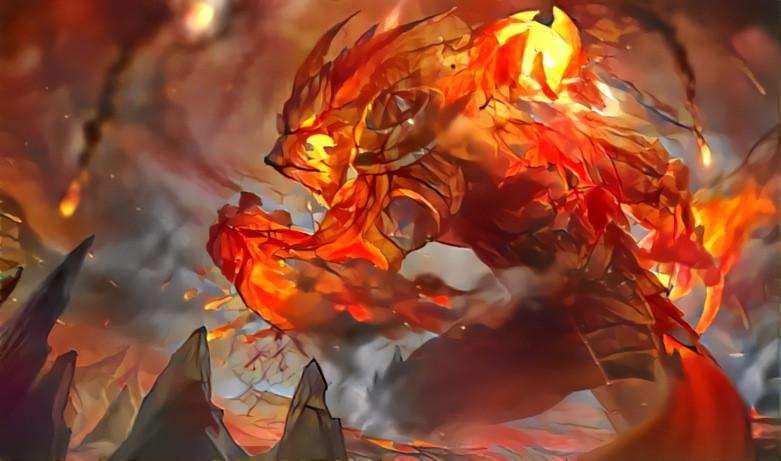
\includegraphics[width=\linewidth]{Graphics/Herbstfang.jpg}
  \caption{\cite{mylatex}\\Another picture}\label{fig:AutumnCatch2}
\endminipage\hfill
\minipage{0.32\textwidth}
  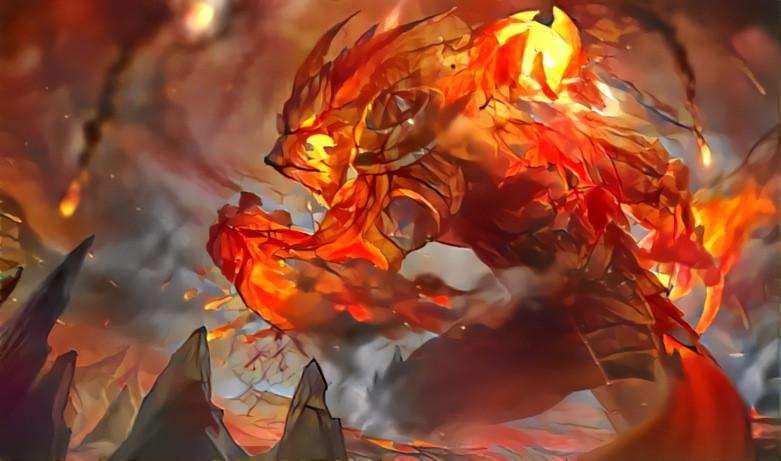
\includegraphics[width=\linewidth]{Graphics/Herbstfang.jpg}
  \caption{\cite{mylatex}\\Yet another picture}\label{fig:AutumnCatch3}
\endminipage\hfill
\minipage{0.32\textwidth}%
  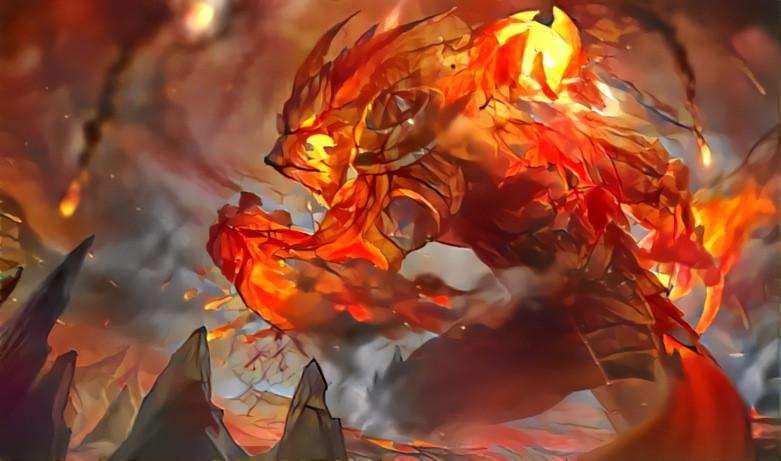
\includegraphics[width=\linewidth]{Graphics/Herbstfang.jpg}
  \caption{\cite{mylatex}\\And \textbf{yet} another picture}\label{fig:AutumnCatch4}
\endminipage
    \end{figure}
    \FloatBarrier
    \noindent

\newpage
\subsection{PDF Page}
\begin{figure}[ht]
    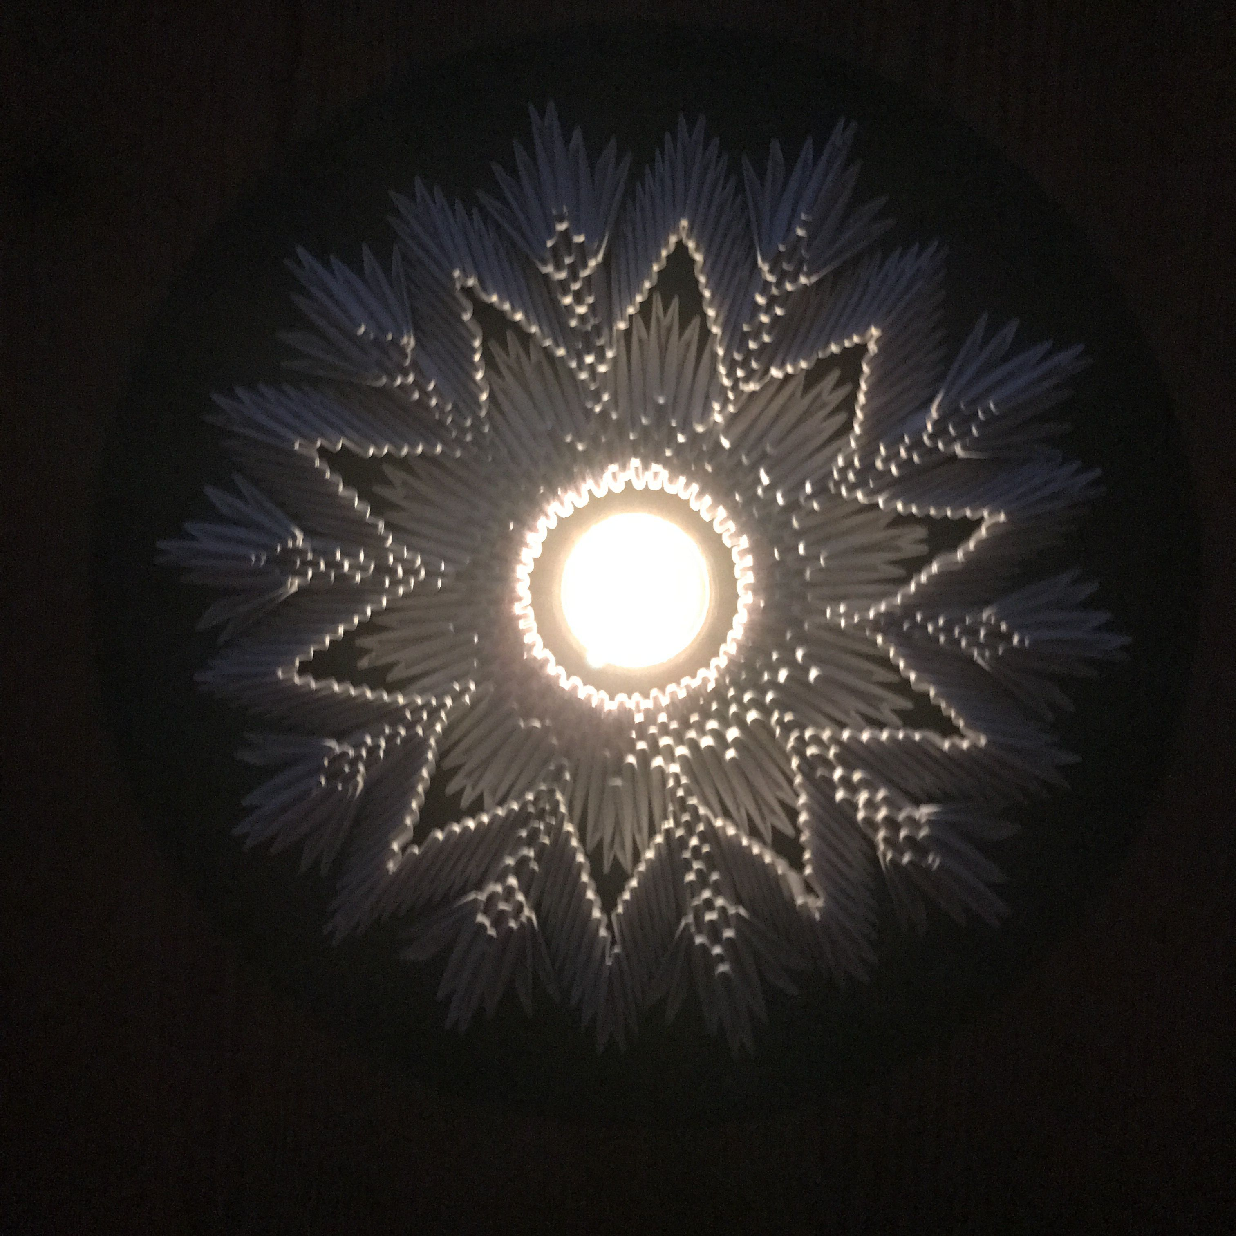
\includepdf[pages=1, width=\textwidth]{Misc/Tangrami.pdf}
    \caption{Some PDF file}
    \label{fig:Tangrami}
\end{figure}
\FloatBarrier
\noindent
\newpage

\section{Tables}
\subsection{Random}
\noindent
\FloatBarrier
\begin{table}[htbp]
    \centering
    \caption{Example table with fixed and variable column widths}
    \begin{tabular}{|>{\centering\arraybackslash}p{2cm}|c|c|p{3cm}|}
        \hline
        \multicolumn{2}{|c|}{\textbf{Fixed Width}} & \multicolumn{2}{c|}{\textbf{Variable Width}} \\
        \hline
        \textbf{Col 1} & \textbf{Col 2} & \textbf{Col 3} & \textbf{Col 4} \\
        \hline
        Row 1 & Content & Content & Some long content that wraps within the specified width \\
        \hline
        Row 2 & Content & Content & Some long content that wraps within the specified width \\
        \hline
    \end{tabular}
    \label{tab:example}
\end{table}
\FloatBarrier
\subsection{Truth Table}
Here is the table \ref{tab:IDK}
\noindent
\FloatBarrier
\begin{table}[ht]
    \centering
    \caption{Logic Table}
    \begin{tabular}{@{ }c@{ }@{ }c@{ }@{ }c | c@{ }@{}c@{}@{ }c@{ }@{ }c@{ }@{ }c@{ }@{ }c@{ }@{ }c@{ }@{}c@{}@{ }c@{ }@{}c@{}@{ }c@{ }@{ }c@{ }@{ }c@{ }@{ }c@{ }@{ }c@{ }@{}c@{}@{ }c}
        \emph{A} & \emph{B} & \emph{C} &  $\emph{D}=$ & ( & $\lnot$ & \emph{A} & $\land$ & $\lnot$ & \emph{C} & ) & $\lor$ & ( & $\lnot$ & \emph{B} & $\land$ & $\lnot$ & \emph{C} & ) & \\
        \hline
        1 & 1 & 1 &  &  & 0 & 1 & 0 & 0 & 1 &  & \textcolor{red}{0} &  & 0 & 1 & 0 & 0 & 1 &  & \\
        1 & 1 & 0 &  &  & 0 & 1 & 0 & 1 & 0 &  & \textcolor{red}{0} &  & 0 & 1 & 0 & 1 & 0 &  & \\
        1 & 0 & 1 &  &  & 0 & 1 & 0 & 0 & 1 &  & \textcolor{red}{0} &  & 1 & 0 & 0 & 0 & 1 &  & \\
        1 & 0 & 0 &  &  & 0 & 1 & 0 & 1 & 0 &  & \textcolor{red}{1} &  & 1 & 0 & 1 & 1 & 0 &  & \\
        0 & 1 & 1 &  &  & 1 & 0 & 0 & 0 & 1 &  & \textcolor{red}{0} &  & 0 & 1 & 0 & 0 & 1 &  & \\
        0 & 1 & 0 &  &  & 1 & 0 & 1 & 1 & 0 &  & \textcolor{red}{1} &  & 0 & 1 & 0 & 1 & 0 &  & \\
        0 & 0 & 1 &  &  & 1 & 0 & 0 & 0 & 1 &  & \textcolor{red}{0} &  & 1 & 0 & 0 & 0 & 1 &  & \\
        0 & 0 & 0 &  &  & 1 & 0 & 1 & 1 & 0 &  & \textcolor{red}{1} &  & 1 & 0 & 1 & 1 & 0 &  & \\
    \end{tabular}
    \label{tab:IDK}
\end{table}
\FloatBarrier
\section{Code}
Here is a code listing \ref{lst:example} using lstlisting.
% example for a code-listing
% Add \hspace{10cm} in front of the \begin if used in combination with \item
% Add '\newpage' to the end of a line for a page break
\begin{lstlisting}[language=C, caption={Example Code}, label=lst:example, breaklines=true, escapeinside='']
#include <stdio.h>

int main() {
    printf("Hello, World!\n");
    return 0;
}
\end{lstlisting}

\section{Idk}
\begin{align*}
    z_0*/z_1*/z_2*/mreq + z_0*/z_1*/z_2*/a_{31} + /z_0*/z_1*z_2*/mreq + /z_0*z_1*z_2*/mreq = z_0' \\
    z_0*/z_1*/z_2*mreq*mw*a31 + /z_0*z_1*/z_2 + /z_0*z_1*z_2*mreq = z_1' \\
    /z_0*/z_1*z_2*mreq + /z_0*z_1*/z_2 + /z_0*z_1*z_2*mreq + /z_0*z_1*/z_2 = z_2' \\
    /z_0*z_1*/z_2+/z_0*z_1*/z_2 = /SMack \\
    /z_0*z_1*/z_2+/z_0*/z_1*z_2 = /SDdoe \\
    /z_0*z_1*/z_2 = /SMw
\end{align*}

\section{Plots}
\subsection{Simple Plot}
\noindent
\FloatBarrier
\begin{figure}[ht]
        \centering
        \begin{tikzpicture}
          \begin{axis}[ 
            xlabel=$x$,
            ylabel={$f(x) = x^3 + \sin(5x^2)$}
          ] 
            \addplot {x^3 + sin(5*x^2)}; 
          \end{axis}
        \end{tikzpicture}
        \caption{A simple plot}
        \label{fig:simpleplot}
\end{figure}
\FloatBarrier

\subsection{A Simple 3D Plot}
\noindent
\FloatBarrier
\begin{figure}[ht]
        \centering
        \begin{tikzpicture}
            \begin{axis}[ 
            xlabel=$x$,
            ylabel=$y$,
            zlabel=$z$
            ] 
            \addplot3 coordinates 
            {
                (0,0,1)
                (0,1,0)
                (0,0,-1)
                (0,-1,0)
                (1,0,0)
            };
            \end{axis}
        \end{tikzpicture}
        \caption{A 3D plot}
        \label{plt:3dplot}
\end{figure}

\section{Manually Created Chart}
\pgfplotstableread[row sep=\\,col sep=&]{
    interval & carT\\
    100     & 0\\
    200     & 2\\
    300    & 5\\
    400   & 35\\
    500   & 40\\
    600     & 45\\
    700     & 25\\
    800     & 15\\
    900     & 0\\
    }\mydata
\noindent
\FloatBarrier
\begin{figure}[ht]
        \centering
        \begin{tikzpicture}
            \begin{axis}[
                    ybar,
                    bar width=.5cm,
                    width=\textwidth,
                    height=.5\textwidth,
                    legend style={at={(0.5,1)},
                        anchor=north,legend columns=-1},
                    symbolic x coords={100,200,300,400,500,600,700,800,900,},
                    xtick=data,
                    nodes near coords,
                    nodes near coords align={vertical},
                    ymin=0,ymax=60,
                    ylabel={Number of artifacts},
                    xlabel={RV},
                ]
                \addplot table[x=interval,y=carT]{\mydata};
                %\addplot table[x=interval,y=carD]{\mydata};
                %\addplot table[x=interval,y=carR]{\mydata};
                \legend{Artifacts}
            \end{axis}
        \end{tikzpicture}
        \caption{A slightly less simple plot} 
        \label{fig:notsimpleplot}
\end{figure}
\FloatBarrier

\section{Piechart}
\begin{tikzpicture}
\pie{22.97/Los Angeles Lakers,
    22.97/Boston Celtics,
    8.11/Golden State Warriors,
    8.11/Chicago Bulls,
    6.76/San Antonio Spurs,
    31.07/Other Teams}
\end{tikzpicture}

\section{Controller}
I pressed the \controllerbutton{A} button to confirm my choice. Then, I pressed the \controllerbutton{B} button to cancel the operation.

\section{Citations}
\subsection{Quotations}
\subsubsection{Inline}
I think \textquote{Never change a running system} is one of the worst takes I can think of.
\subsection{Referencing}
\cite{etechformelsammlung}
\newpage

\section{External Tools / Useful Links}
\begin{itemize}
    \item \href{https://detexify.kirelabs.org/classify.html}{Detexify - Find symbol command names by drawing them}
    \item \href{https://texample.net/tikz/examples/}{Tikz examples (categorized)}
    \item \href{https://www.bibtex.com/e/entry-types/}{Bibtex entry types}
    \item \href{https://latexdraw.com/three-dimensional-plotting-in-latex/}{Complex 3D plotting}
    \item \href{https://mirror.informatik.hs-fulda.de/tex-archive/info/lshort/english/lshort.pdf}{The not so short Introduction to \LaTeX}
    \item \href{https://en.wikibooks.org/wiki/LaTeX}{Where to find even more references}
\end{itemize}

\newpage
\printbibliography[heading=bibintoc] % if you have biblatex included
\end{document}

